% !TEX encoding = UTF-8
\section{导言}
这里是导言,这里是导言,这里是导言。这里是导言,这里是导言,这里是导言。这里是导
言,这里是导言,这里是导言。这里是导言,这里是导言,这里是导言。这里是导言,这里
是导言,这里是导言。这里是导言,这里是导言,这里是导言。这里是导言,这里是导言,
这里是导言。这里是导言,这里是导言,这里是导言。这里是导言,这里是导言,这里是导
言。这里是导言,这里是导言,这里是导言。这里是导言,这里是导言,这里是导言。
%第一章
\section{机器学习}
\subsection{什么是机器学习}
%什么是机器学习
\par 
什么是机器学习,什么是机器学习,什么是机器学习,什么是机器学习什么是机器学习,什
么是机器学习什么是机器学习,什么是机器学习什么是机器学习,什么是机器学习什么是机
器学习,什么是机器学习什么是机器学习,什么是机器学习什么是机器学习,什么是机器学
习\cite{机器学习技术的应用经验及建议探讨}。

%机器学习算法
\subsection{常见的机器学习方法}
%K-means算法
\subsubsection{K-means算法}
\par 
K-means,K-means,K-means,K-means,K-means,K-means,K-means,K-means,K-means,K-means,K-me
ans,K-means,K-means,K-means,K-means,K-means,
%聚类是非监督学习的一种形式,它将一个观测集(即数据点)划分到孜然组合或者模式划分到
自然组或者模式聚类,聚类的途径是测量分配给每个聚类的观测对之间的相似性以最小一个指
定的代价函数\cite{Simon2011神经网络与机器学习}。

\begin{equation}
	C\left(i\right) = arg \min_{i \le j \le K}    \Vert \mathbf{x_i}  - \hat{\mathbf{\mu_j}} \Vert^{2}  
\end{equation}
	
%%tikz绘图
\begin{figure}[h]
	\centering
	\begin{tikzpicture}
		\node (ciji)  [] at (-0.5,0) {刺激};
		\node (ganshouqi)[draw,minimum height = 0.8cm,thick] at (1.5,0)  {感受器};
		\node (shenjing)    [draw,minimum height = 0.8cm,thick]  at (4,0) {神经网络};
		\node (xiaoying)   [draw,minimum height = 0.8cm,thick] at (6.5,0) {效应器};
		\node (xiangying) [minimum height = 0.8cm,thick] at (8.5,0) {响应};
		\draw [-Stealth]  (ciji.east) -- (ganshouqi.west);
		\draw [-Stealth] (2.172,0.2) -- (3.146,0.2);
		\draw [-Stealth] (3.146,-0.2) -- (2.172,-0.2);
		\draw [-Stealth] (4.87,0.2) -- (5.83,0.2);
		\draw [-Stealth] (5.83,-0.2) -- (4.87,-0.2);
		\draw [-Stealth] (xiaoying.east) -- (xiangying.west); 
	\end{tikzpicture}
	\caption{神经系统}
	\label{neutural network}
\end{figure}

\begin{figure}[htbp]
	\centering
	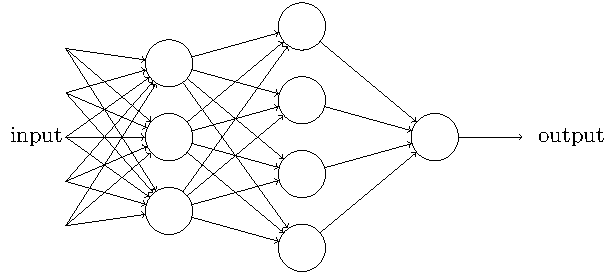
\includegraphics{Neural Networks-pic1.pdf}
	\caption{神经网络}
	\label{Neural Networks}
\end{figure}

